\documentclass[12pt,a4paper]{article}

% -------------------
% MARK: Packages
% -------------------

% import geometry package to update the document margins
\usepackage[margin=1in]{geometry}
% set the font to helvectica
\usepackage[scaled]{helvet}
\renewcommand\familydefault{\sfdefault}
% for type-setting
\usepackage{amsmath, amssymb, amsfonts, verbatim, pifont}
% for slashed out text
\usepackage[normalem]{ulem}
% for units and scientific notation
\usepackage[table]{xcolor}
\usepackage{siunitx}
% for references and URLs
\usepackage{hyperref, url}
% Natbib setup for author-year style
\usepackage{natbib}
 \bibpunct[, ]{(}{)}{,}{a}{}{,}%
 \def\bibfont{\small}%
 \def\bibsep{\smallskipamount}%
 \def\bibhang{24pt}%
 \def\newblock{\ }%
 \def\BIBand{and}%
% for graphics and figures
\usepackage{graphicx, subfig, tikz}
% force figures to stay in their sections
\usepackage[section]{placeins}
% for tables
\usepackage{booktabs, longtable, tabularx}
\usepackage{multicol, multirow}
\usepackage{adjustbox}
\usepackage[flushleft]{threeparttable}
% a package for working with .csv data for tables
\usepackage{csvsimple}
% setup the algorithm package
% ruled: show bars around title and bar at bottom
% lined: show the line column on the left of the algorithm
% linesnumbered: print line numbers for each line
\usepackage[ruled,lined,linesnumbered]{algorithm2e}
\DontPrintSemicolon % don't print the semicolon that \; usually prints
% fix overfull hbox errors from oddities like using
% quotes (``foo'') and etc.
\usepackage{microtype}

% -------------------
% MARK: Debugging Packages
% -------------------

% import a debugging package to show the margin boxes
% \usepackage{showframe}

% -------------------
% MARK: Declarations
% -------------------

% setup captions for tables and figures
\captionsetup[table]{%
  labelfont={bf},
  name={Table},
  labelsep=colon,
  justification=raggedright,
  singlelinecheck=false}
\captionsetup[figure]{%
  labelfont={bf},
  name={Figure},
  labelsep=colon,
  justification=raggedright,
  singlelinecheck=false}
\captionsetup[algorithm2e]{%
  labelfont={bf},
  name={Figure},
  labelsep=colon,
  justification=raggedright,
  singlelinecheck=false}

% set the graphics path to the img directory
\graphicspath{{img/}}

% -----------------------------------------------------------------------------
% MARK: algorithm2e stuff
% -----------------------------------------------------------------------------

% params
% \SetKwInOut{Objects}{$\CKmatrix{O}$}
% \SetKwInOut{Weights}{$\CKvector{w}$}

% -------------------
% MARK: Headers
% -------------------

% headers and footers
\usepackage{fancyhdr}
\setlength{\headheight}{15pt}
\pagestyle{fancy}
\lhead{KautenjaDSP}
\rhead{\itshape POKEY v1.6.0}
\cfoot{\thepage}

% start the document
\begin{document}

% -------------------
% MARK: Title Page
% -------------------

% fancyhdr directive to remove headers from this title page
\thispagestyle{empty}
% center the title page contents
\vspace*{\fill}
\begin{center}

\includegraphics{POKEY-Logo}
\linebreak\linebreak\linebreak\linebreak
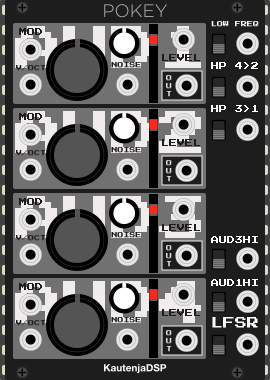
\includegraphics{POKEY-Module}
\linebreak\linebreak\linebreak\linebreak

\includegraphics{KautenjaDSP}
\end{center}
\vspace*{\fill}
\clearpage

% -------------------
% MARK: Overview
% -------------------

\section{Overview}

POKEY is an emulation of the Atari POKEY audio processing unit. The POKEY
produces four pulse waveforms, but contains a variety of bonus controls,
including extended frequency ranges, high-pass filters, and noise generators /
distortion effects.

POKEY provides the key features of the POKEY chip, namely,
\begin{itemize}
  \item \textbf{Quad pulse wave generator:} Four pulse waves with 8-bit frequency value and $50\%$ pulse width
  \item \textbf{Low-frequency mode:} Change base clock of the chip from $64 KHz$ to $15 KHz$
  \item \textbf{High-frequency mode:} Change base clock of channels 1 and 3 from $64 KHz$ to $1.79 MHz$
  \item \textbf{High-pass filter:} High-pass filter channel 1 using channel 3 as a clock or high-pass channel 2 using channel 4 as a clock
  \item \textbf{Linear Feedback Shift Register (LFSR):} old-school 8-bit randomness!
  \item \textbf{Noise/Distortion generator:} generate per-channel pseudo-random numbers at 15 different frequencies as a distortion source
  \item \textbf{Amplitude modulation:} 4-bit amplifier with linear amplitude modulation
\end{itemize}

% -------------------
% MARK: Panel Layout
% -------------------

\clearpage
\section{Panel Layout}
\begin{figure}[!htp]
\centering
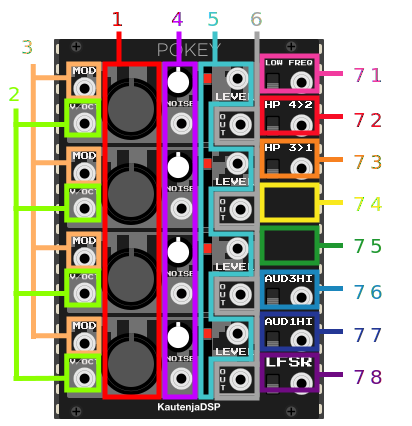
\includegraphics{POKEY-Manual}
\end{figure}

\clearpage
\begin{enumerate}
  \item Coarse frequency control over the each four the pulse waveform generators.
  \item $V$/Octave inputs for each of the four pulse waveform generators.
  \item Linear CV frequency modulation for each of the four pulse waveform generators.
  \item Shift register value for each noise generator $\in [0, 7]$ for the noise generator of each channel. Random numbers are generated by sampling the high 8 bits from the top of the 17-bit shift register. The shift register is clocked by the $1.79MHz$ clock of the chip's CPU. See Table~\ref{tab:shift-register} for a description of each shift register setting.
  \item Coarse amplitude control over each of the channels using 4-bit amplifiers.When no input is connected, the slider controls the level from $0\%$ to $100\%$. When an input is connected, the slider acts as an attenuator.
  \item Channel outputs, ${\approx}10V_{pp}$.
  \item Switch and gate control over each bit in the audio control register. See Table~\ref{tab:audio-control} for descriptions of each of the bits. CV control goes high at $2V$. The switch flips the bit and inverts the effect of the CV input.
\end{enumerate}

\begin{table}[!htp]
\centering
\caption{Shift register values for the noise generators.}
\label{tab:shift-register}
\small
\begin{tabular}{|c||l|}
\hline
Mode & Description                   \\
\hline\hline
 0    & 5-bit then 17-bit polynomials \\
 1    & 5-bit poly only               \\
 2    & 5-bit then 4-bit polys        \\
 3    & 5-bit poly only               \\
 4    & 17-bit poly only              \\
 5    & no poly (pure tone)           \\
 6    & 4-bit poly only               \\
 7    & no poly (pure tone)           \\
\hline
\end{tabular}
\end{table}

\begin{table}[!htp]
\centering
\caption{Descriptions of each of the bits in the Audio Control register.}
\label{tab:audio-control}
\small
\begin{tabular}{|l|l||l|l|l|}
\hline
 Bit & Name              & Description                                            & 0        & 1          \\
\hline\hline
 1   & \texttt{LOW FREQ} & Choice of frequency divider rate for all channels      & $64 kHz$ & $15 kHz$   \\
 2   & \texttt{HP 4>2}   & High-pass filter for Ch. 2 rated by frequency of Ch. 4 & Off      & On         \\
 3   & \texttt{HP 3>1}   & High-pass filter for Ch. 1 rated by frequency of Ch. 3 & Off      & On         \\
 4   & \texttt{16=4+3}   & Combine Ch. 4 \& Ch. 3 to achieve 16-bit frequency     & Off      & On         \\
 5   & \texttt{16=2+1}   & Combine Ch. 2 \& Ch. 1 to achieve 16-bit frequency     & Off      & On         \\
 6   & \texttt{AUD3HI}   & Channel 3 clock divider frequency                      & $64 kHz$ & $1.79 MHz$ \\
 7   & \texttt{AUD1HI}   & Channel 1 clock divider frequency                      & $64 kHz$ & $1.79 MHz$ \\
 8   & \texttt{LFSR}     & Noise / distortion shift register                      & 17-bit   & 9-bit      \\
\hline
\end{tabular}
\end{table}

% -------------------
% MARK: References
% -------------------

\clearpage
\renewcommand\refname{References \& Acknowledgments}
\nocite{*}
\bibliographystyle{apalike}
\bibliography{references}

\end{document}
